\documentclass[12pt]{article}
\usepackage{sbc-template}
\usepackage{graphicx,url}
\usepackage[brazil]{babel}   
%\usepackage[latin1]{inputenc}  
\usepackage[utf8]{inputenc}  
% UTF-8 encoding is recommended by ShareLaTex
%%%%resolver numeração
\usepackage{etoolbox}
\makeatletter
\patchcmd{\ttlh@hang}{\parindent\z@}{\parindent\z@\leavevmode}{}{}
\patchcmd{\ttlh@hang}{\noindent}{}{}{}
\makeatother
%%%%%%%
\sloppy

\author{Matheus R. A. Melo\inst{1}, Monaly V. Correia\inst{1}, Paulo H. R. Abreu\inst{1}, Elthon A. Oliveira\inst{1}}
\address{
   Universidade Federal de Alagoas - \textit{Campus} Arapiraca\\
   Núcleo de Ciências Exatas (NCEX)\\
   Laboratório Multidisciplinar de Computação / Coletivo EIDI    
  \email{matheus.melo@arapiraca.ufal.br, monaly\textunderscore vital@hotmail.com,} \email{paulo.abreu@arapiraca.ufal.br, elthon@arapiraca.ufal.br}
}

\title{Uma ferramenta para melhoria da eficiência das ações do Conselho Tutelar do município de Arapiraca}

\begin{document} 

\maketitle

\begin{abstract}
The Tutelar Council operates in Brazil as a municipal body and aims to serve children and adolescents. In the municipality of Arapiraca, the Tutelary Council works with paper processes, which makes its activities inefficient. Such inefficiency reflects negatively on the quality of the services rendered. This article aims to present the development of a system for the Tutelary Council of the municipality of Arapiraca. Such a system aims to computerize the processes of registration of occurrences, consultations and generation of reports. In this way, it is expected to improve the efficiency of care for this vulnerable part of the population that is made up of children and adolescents.
\end{abstract}
     
\begin{resumo}
Conselho Tutelar atua no Brasil como órgão municipal e tem por objetivo atender crianças e adolescentes. No município de Arapiraca, o Conselho Tutelar trabalha com processos de papel, o que torna suas atividades ineficientes. Tal ineficiência reflete negativamente na qualidade dos atendimentos feitos. Este artigo tem como objetivo apresentar o desenvolvimento de um sistema para o Conselho Tutelar do município de Arapiraca. Tal sistema objetiva informatizar os processos de cadastro de ocorrências, consultas e geração de relatórios. Desta forma, espera-se melhorar a eficiência no atendimento a esta parcela tão vulnerável da população que é formada por crianças e adolescentes.
\end{resumo}


\section{Introdução}
Criado no Ano de 1990, junto ao Estatuto da Criança e do Adolescente, o Conselho Tutelar atua no Brasil como órgão municipal e tem por objetivo atender crianças e adolescentes, aplicando as medidas cabíveis. Ele também tem por objetivo atender e/ou aconselhar pais ou responsáveis, executando as medidas adequadas, bem como encaminhar ao Ministério Público infrações administrativas ou penais contra os direitos da criança e do adolescente. 

Além disso, é função do Conselho Tutelar providenciar a medida estabelecida pela autoridade judiciária para o adolescente autor do ato infracional, representar, em nome da pessoa e da família, contra a violação de direitos previstos na Constituição Federal, dentre outros mais. O conselho tutelar é autônomo em suas decisões. O mesmo tem o poder de determinar medidas e as mesmas não serem interferidas por órgãos externos, fazendo com que não haja uma relação de subordinação com qualquer órgão do estado. Todavia, o Conselho tutelar não tem autonomia de aplicar qualquer medida que caiba a esfera jurídica do processo em andamento.

No município de Arapiraca, o Conselho tutelar é dividido em dois polos denominados região 1 e região 2, os quais atendem a uma determinada área da cidade cada. Como sua função contempla o registro de ocorrências, a consulta de processos (em aberto ou finalizados), geração de relatórios, dentre outros, o Conselho Tutelar necessita de algum mecanismo que gerencie de forma eficiente tais procedimentos. Até então, o Conselho Tutelar do município de Arapiraca utilizava exclusivamente fichas de papel arquivadas em armários e pastas, como apresentado na Figura~\ref{fig:arquivos}. Este modelo de funcionamento faz com que o trabalho se torne bastante ineficiente. Em algumas situações vividas pelos conselheiros, demandavam-se horas, ou até dias, para executar determinados procedimentos.

\begin{figure}[ht]
\centering
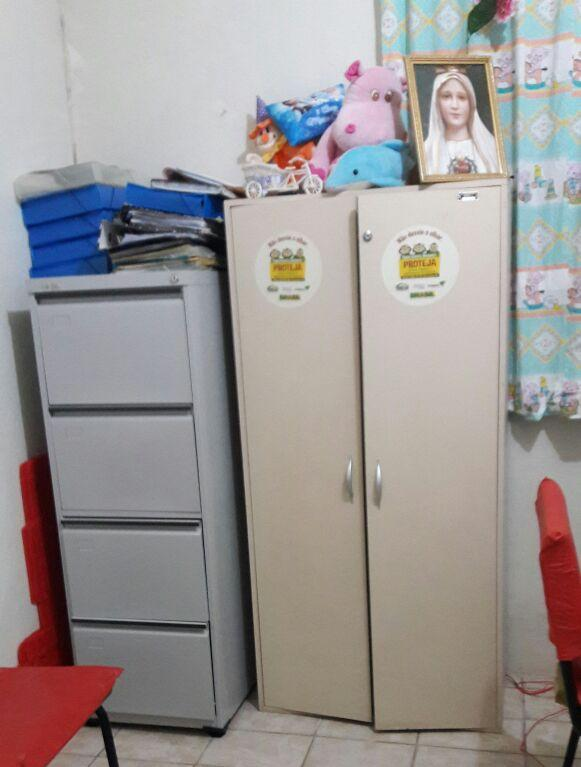
\includegraphics[width=.27\textwidth]{fig/1.jpg}
\caption{Processos de papel arquivados no Conselho Tutelar.}
\label{fig:arquivos}
\end{figure}

Uma alternativa criada pelo governo federal foi o sistema denominado SIPIA, que tem como função o cadastro de ocorrências e consultas. Entretanto, segundo os conselheiros, o sistema recorrentemente apresenta lentidão ao se fazer o cadastro e/ou consulta de ocorrências. Além disso, ainda segundo os conselheiros, o SIPIA apresenta muita instabilidade, o que o torna inviável de ser utilizado. Outro problema apontado é o constante problema de conexão com a internet existente no Conselho Tutelar do município de Arapiraca. Estes problemas juntos fizeram com que os conselheiros optassem por recorrer aos processos de papel para que as atividades do Conselho continuassem a funcionar, mesmo que de forma ineficiente.

Diante deste cenário, é proposta a criação de um sistema web para o Conselho Tutelar do município de Arapiraca. Este sistema deverá atender a todos os requisitos necessários para um bom funcionamento do serviço por eles oferecidos. É pretendido facilitar o cadastro e consulta de ocorrências por meio da informatização deste processo. Este sistema possibilitará o uso de uma base de dados local e um mecanismo de sincronização com outra base na nuvem. Desta forma, possíveis problemas de conexão com a Internet não inviabilizarão todas as atividades do Conselho.

Ao longo deste artigo são apresentados quais materiais estão sendo utilizados, assim como os métodos aplicados no desenvolvimento do sistema, o que inclui a interação com os usuários (conselheiros) para correção de potenciais \textit{bugs} e adição de novas funcionalidades, quando necessário. 

\section{Materiais e métodos} 

Nesta seção são apresentados as tecnologias usadas no desenvolvimento da ferramenta, bem como a metodologia empregada entre os desenvolvedores e os usuários finais.

\subsection{Materiais}
Neste trabalho são utilizadas algumas tecnologias. Para a parte \textit{back-end}, tem sido utilizada a linguagem PHP com orientação a objetos, pois, favorece o reuso e modularização do código \cite{PHP}. Já a parte \textit{front-end} tem sido desenvolvida utilizando HTML5, CSS e Javascript. Tem sido utilizado o padrão arquitetural MVC (\textit{Model-View-Controller}), que tem favorecida a divisão de tarefas entre os desenvolvedores. Para persistência dos dados tem-se usado o gerenciador de banco de dados MySQL.

\subsection{Métodos}
\subsubsection*{Iteração com os usuários}

O desenvolvimento do sistema está acontecendo mediante reuniões mensais com os usuários finais, para que a cada parte entregue possa ser feita uma avaliação por parte do usuário e a partir disso, a equipe de desenvolvimento possa fazer a correção de \textit{bugs} e adicionar novas funcionalidades, caso seja necessário.

Durante as reuniões estão sendo apresentadas propostas de interfaces que possam melhorar a experiência de usuário, juntamente com novas funcionalidades. Entretanto, mesmo havendo o atendimento de novos requisitos, o sistema encontra-se atualmente em fase beta, no qual as funcionalidades prioritárias de cadastro de ocorrência, consultas e geração de relatórios já se encontram em funcionamento para testes.

\subsubsection*{Iteração entre os desenvolvedores}
A comunicação entre a equipe de desenvolvimento tem sido feita tanto por meio da ferramenta Slack\footnote{\url{https://slack.com/}}, como da ferramenta Trello\footnote{\url{https://trello.com/}}, no qual são definidas as funcionalidades a serem implementadas e o desenvolvedor responsável pela funcionalidade. Esta metodologia tem agilizado o desenvolvimento do sistema, pois, expõe as responsabilidades de forma transparente para que não haja sobreposição de tarefas entre os membros da equipe de desenvolvimento. Reuniões quinzenais são realizadas a fim de sincronizar as tarefas atribuídas aos desenvolvedores, bem como atribuir novas tarefas. 

\section{Trabalho correlato}

A principal ferramenta correlata consiste em um sistema \textit{online} criado pelo governo federal para os Conselhos Tutelares do Brasil denominado SIPIA \cite{Sipia}. O sistema tem como objetivo o cadastro de ocorrências, consultas e geração de relatórios.

No SIPIA, o conselheiro primeiramente faz a solicitação de acesso preenchendo um formulário e enviando certos dados para que possa ser verificado no banco de dados do governo. Após verificada a veracidade desses dados, é concedido acesso ao sistema. Feito a solicitação e autorização de uso, o conselheiro pode utilizar todas as funcionalidades que o software tem a oferecer. Porém, os conselheiros do município de Arapiraca relatam que a lentidão do sistema, somado a conexão de internet de baixa qualidade no ambiente de trabalho deles, fez com que o sistema se tornasse difícil de utilizar, tornando as atividades do Conselho impraticáveis.

\section{A ferramenta proposta}
O sistema em desenvolvimento para o Conselho Tutelar do município de Arapiraca\footnote{Disponível em{ \url{http://conselhotutelar.coletivoeidi.com.br}}}, assim como o software SIPIA, é online e tem como objetivo o cadastro de ocorrências, consulta e geração de relatórios. No entanto ele tem o intuito de resolver os problemas relatados pelos conselheiros em relação ao sistema SIPIA. A ferramenta aqui proposta trabalhará com uma base de dados local e uma na nuvem. Um mecanismo de sincronização dos dados também será desenvolvido. Desta forma, o Conselho Tutelar não precisará parar suas atividades no caso de falha na conexão com a Internet.

Na tela de ``Login'' o conselheiro irá inserir seu nome de usuário e sua senha para que possa ter acesso ao sistema, como mostrado na Figura~\ref{fig:login}. Os logins dos conselheiros são guardados em um banco de dados integrado ao software para que se possa ter uma maior segurança de acesso. Na tela ``Home'' (Figura~\ref{fig:home}) há um pequeno tutorial de como se utilizar o sistema, para que o conselheiro possa se nortear de como fazer uso do mesmo em um primeiro contato, como apresentado na Figura~\ref{fig:home}.

\begin{figure}[ht]
\centering
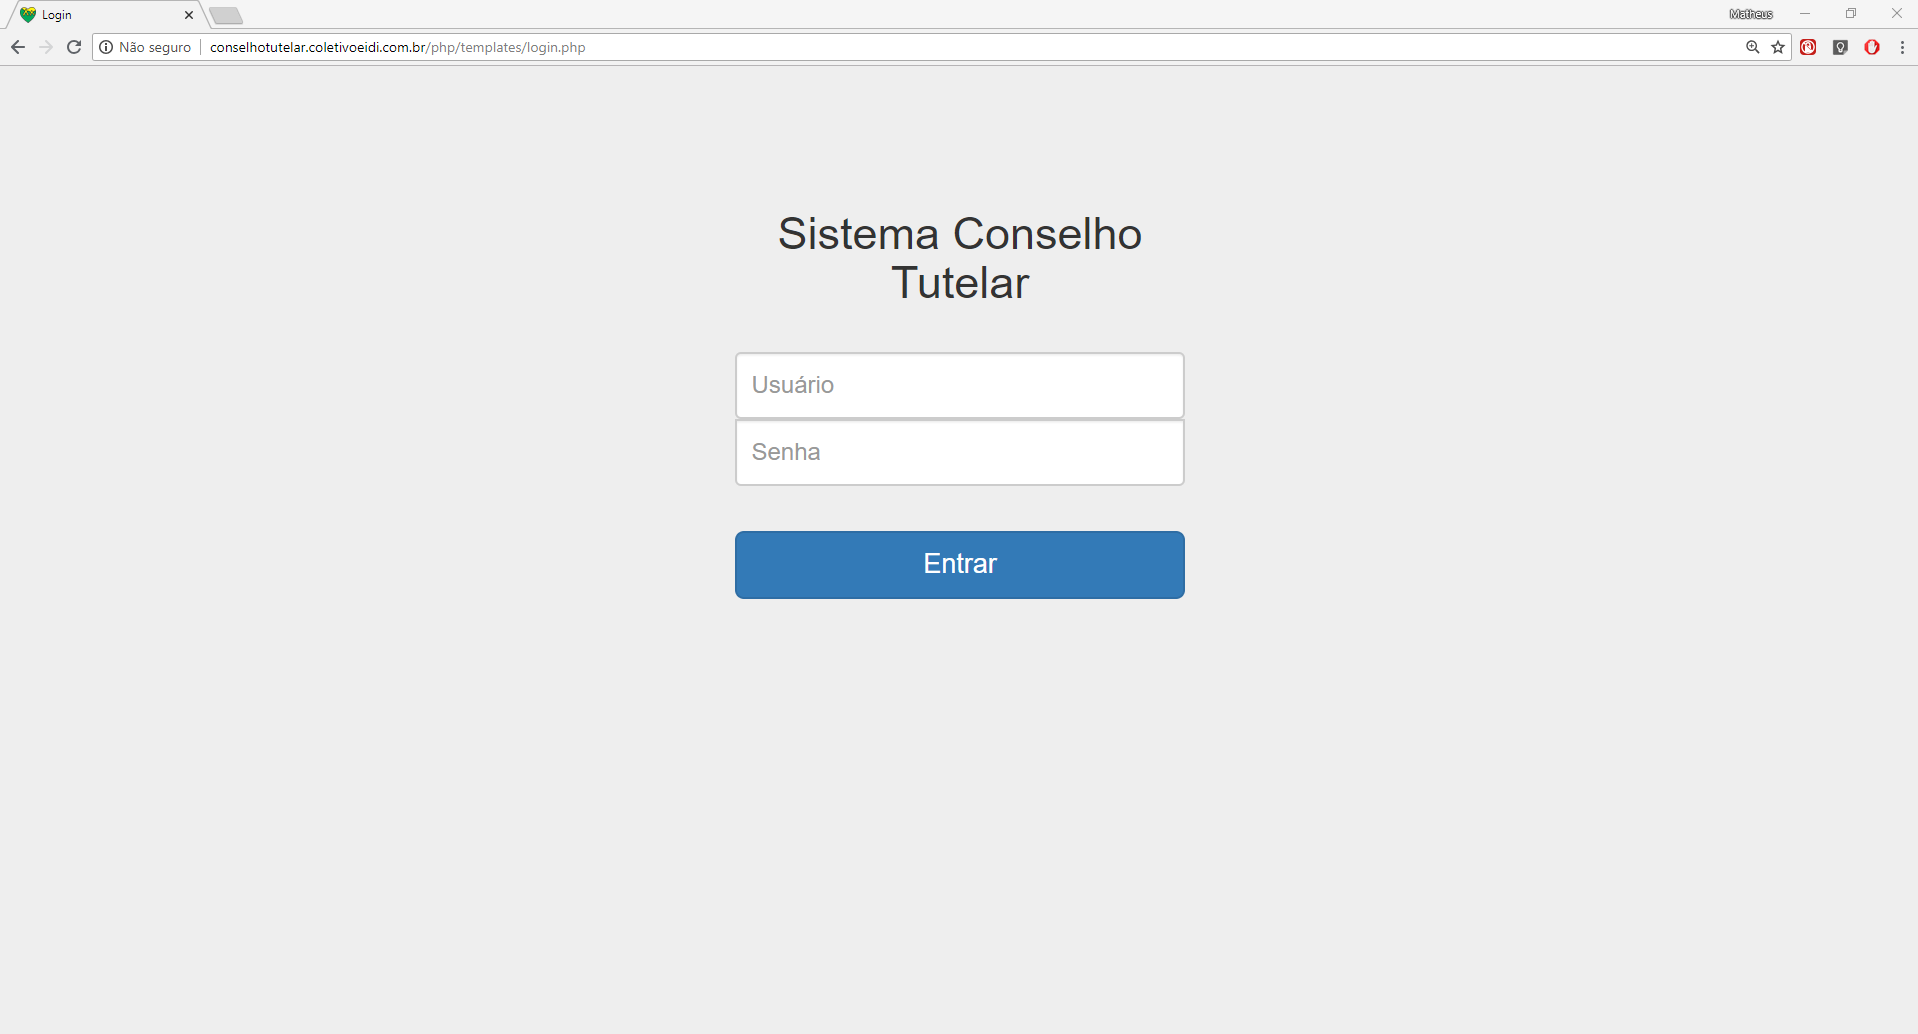
\includegraphics[width=.6\textwidth]{fig/2.png}
\caption{Tela de Login.}
\label{fig:login}
\end{figure}

\begin{figure}[ht]
\centering
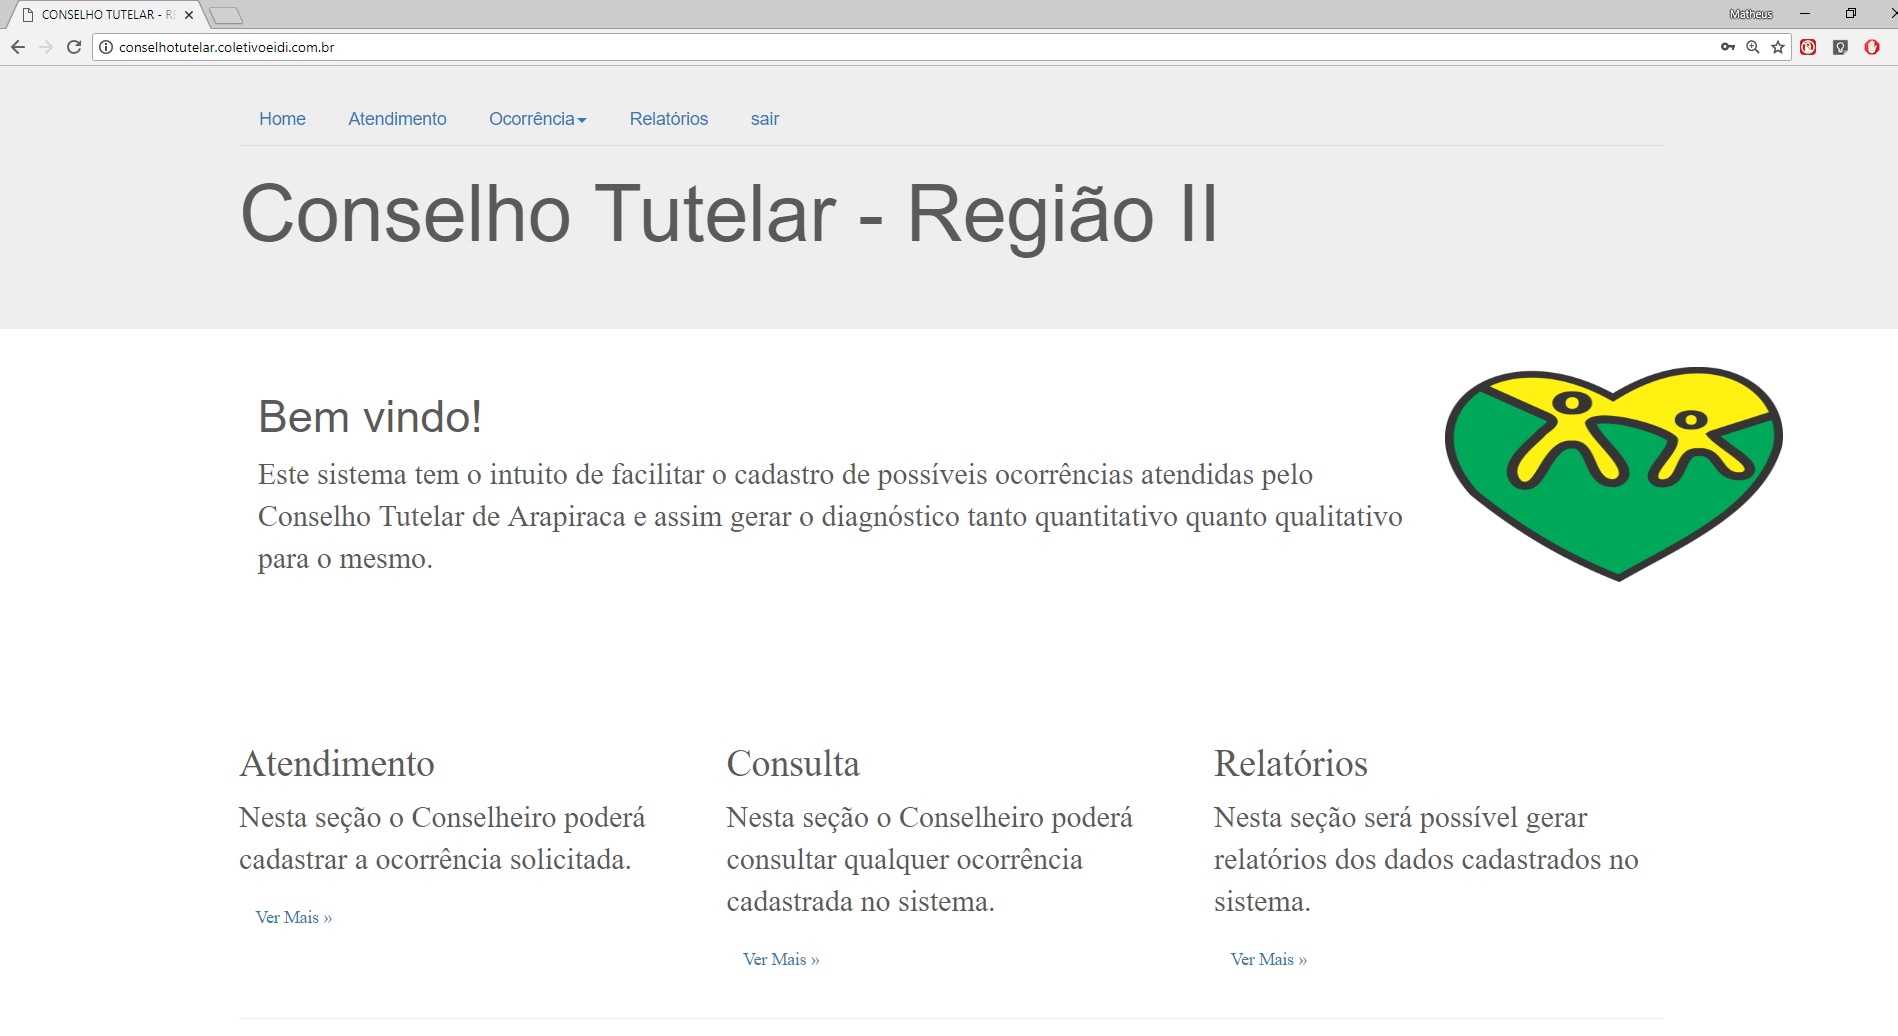
\includegraphics[width=.6\textwidth]{fig/3.png}
\caption{Tela Home.}
\label{fig:home}
\end{figure}

% \begin{figure}[tb]
% \begin{center}
% 	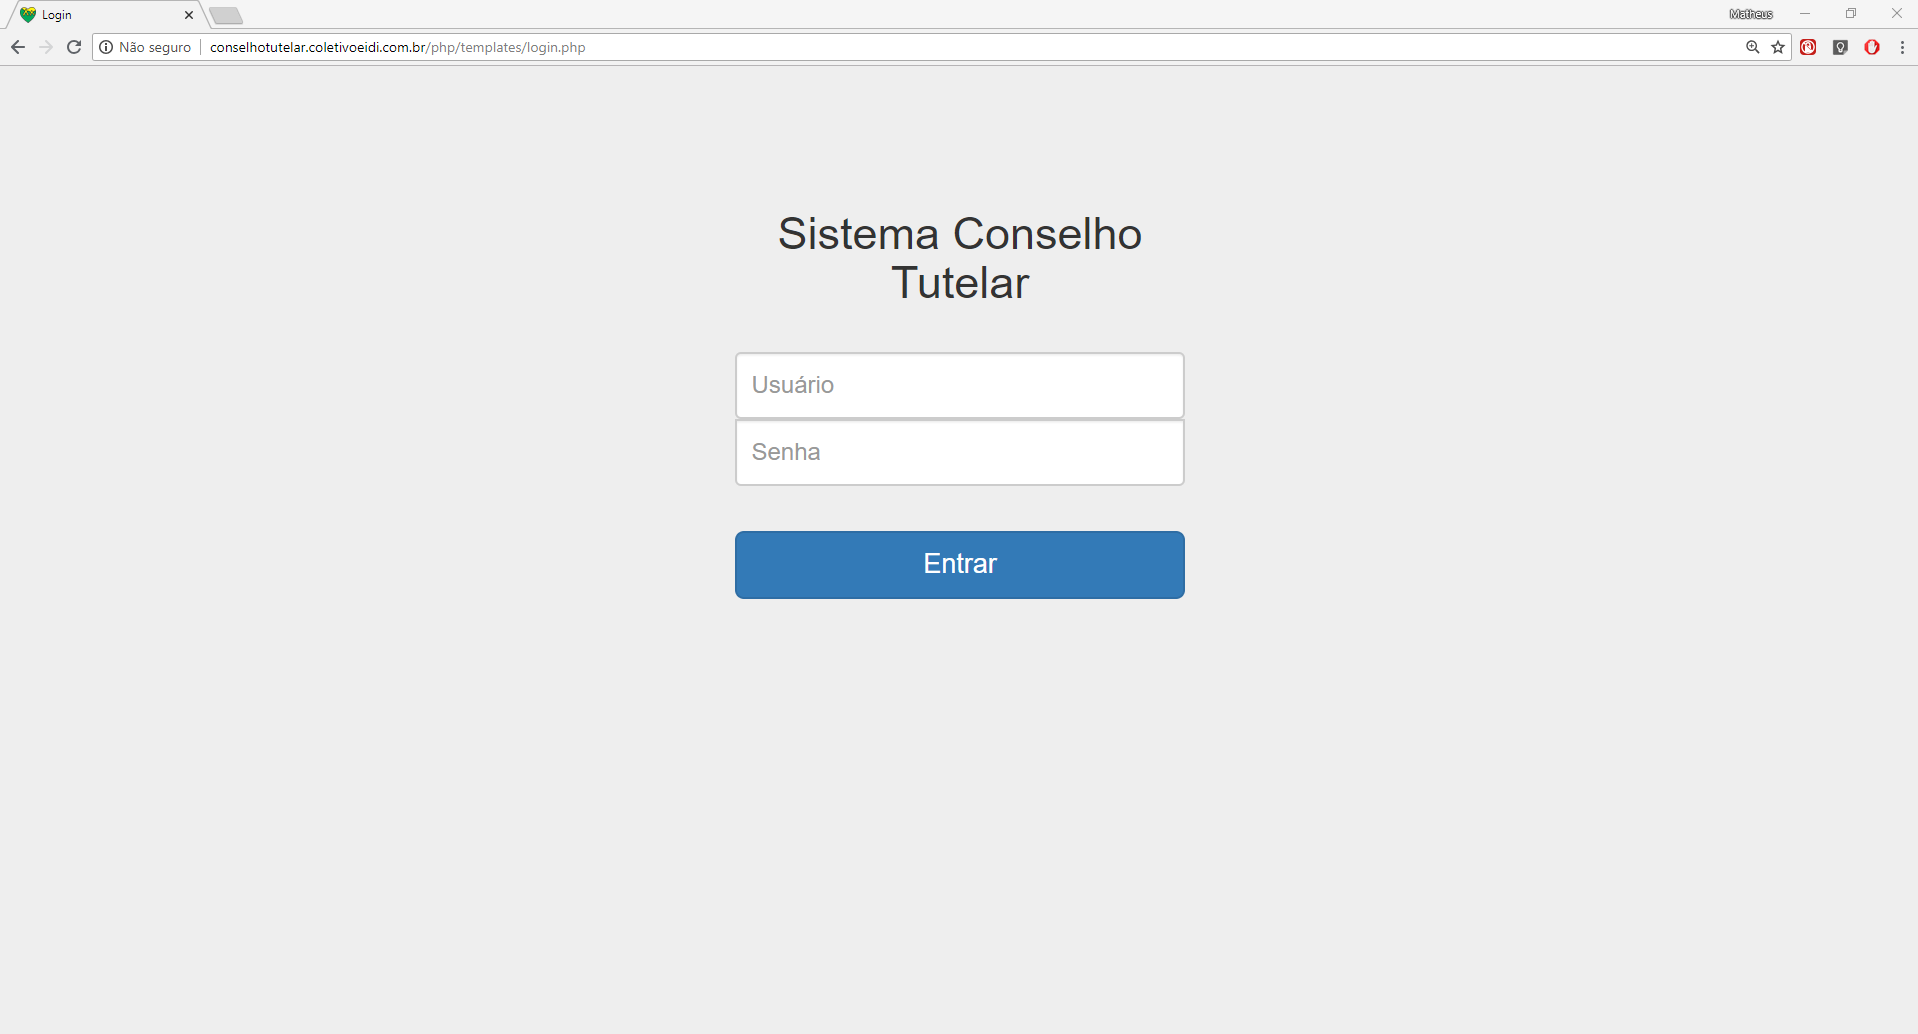
\includegraphics[height=3cm]{fig/2.png} \quad
% 	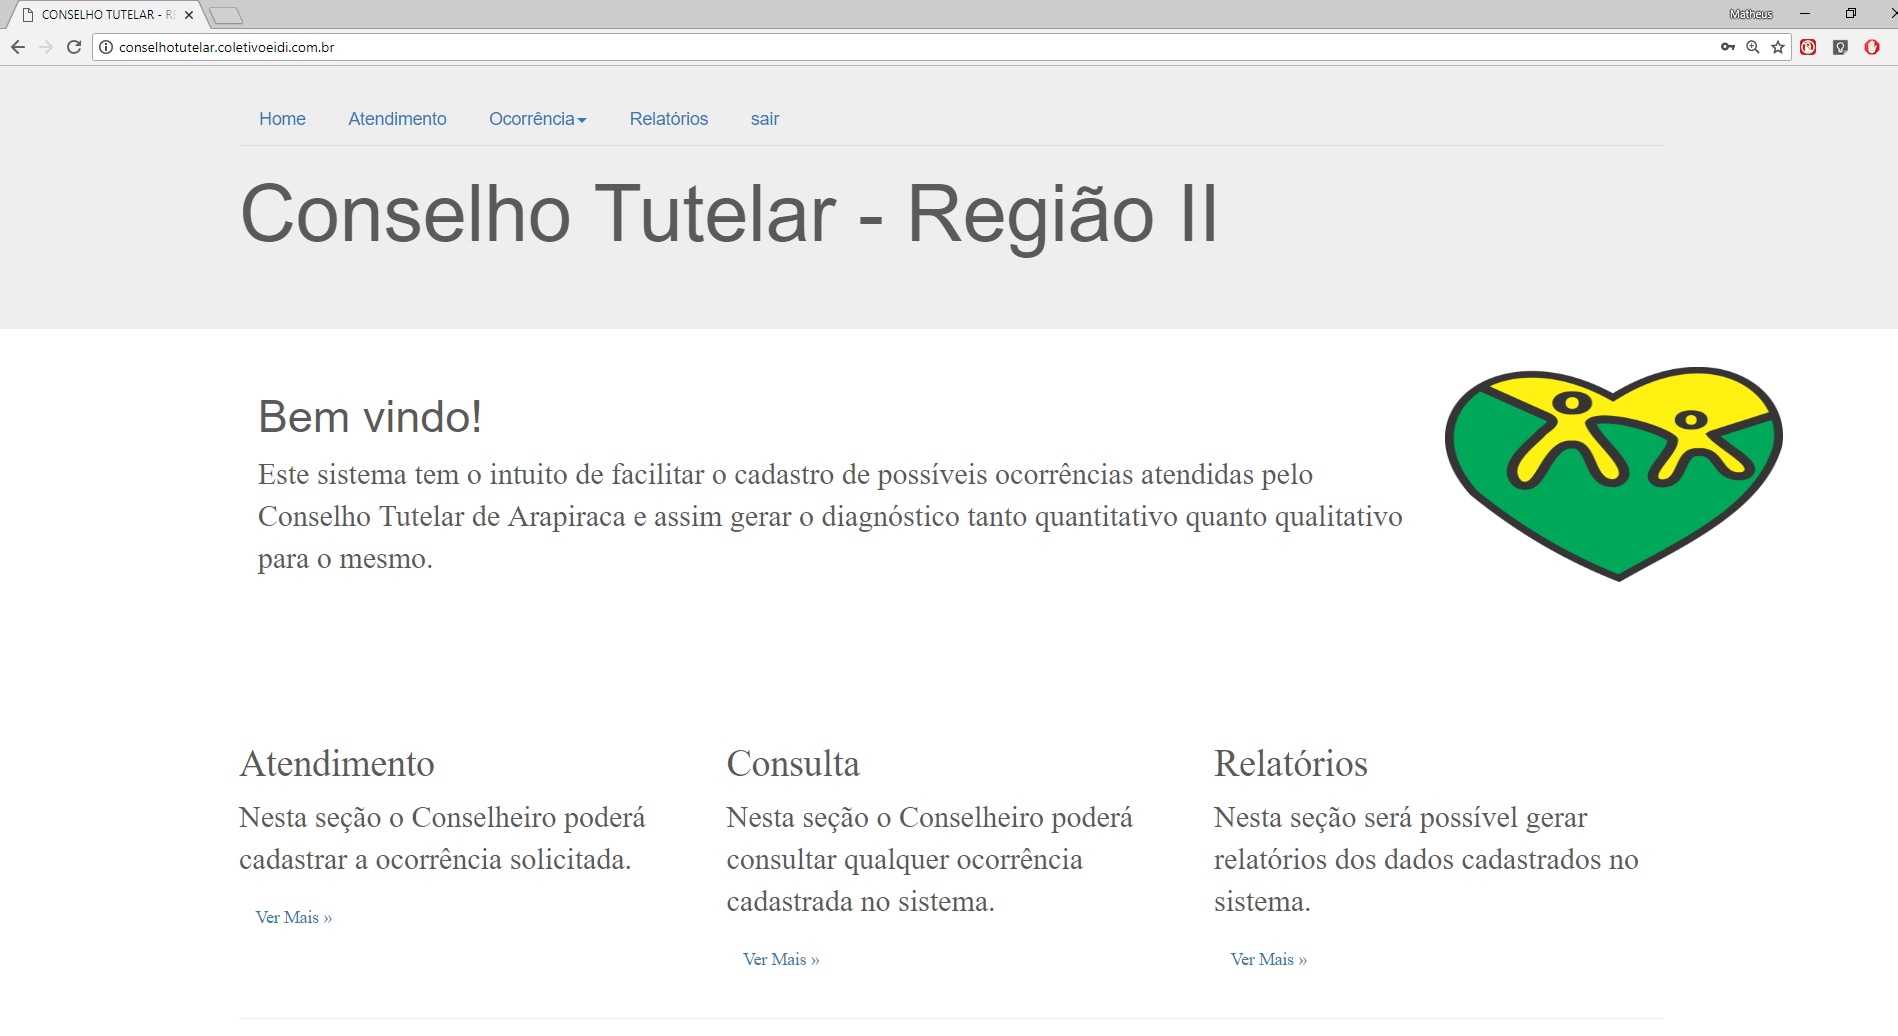
\includegraphics[height=3cm]{fig/3.png}
% \caption{Motes instalados na Great Duck Island} \label{gdimotes}
% \end{center}
% \end{figure}
A tela de ``Atendimento'' (Figura~\ref{fig:atendimento}) é responsável pelo cadastro das ocorrências. Esta tela apresenta um questionário a ser preenchido pelo conselheiro com todos os dados da ocorrência. Tal questionário pode ser preenchido por completo numa única vez ou pode ser preenchido em etapas, caso seja desejado. O questionário apresenta a opção de \textit{conclusão} ou \textit{pendência}, o que possibilita o preenchimento parcial. Caso seja assinalada a opção pendência, o questionário é enviado para aba ``Pendentes'' onde o mesmo poderá ser editado posteriormente. Outra funcionalidade contida no sistema é a geração de PDF da ficha de atendimento. O conselheiro poderá gerar PDFs tanto das fichas de atendimentos quanto dos relatórios.

\begin{figure}[ht]
\centering
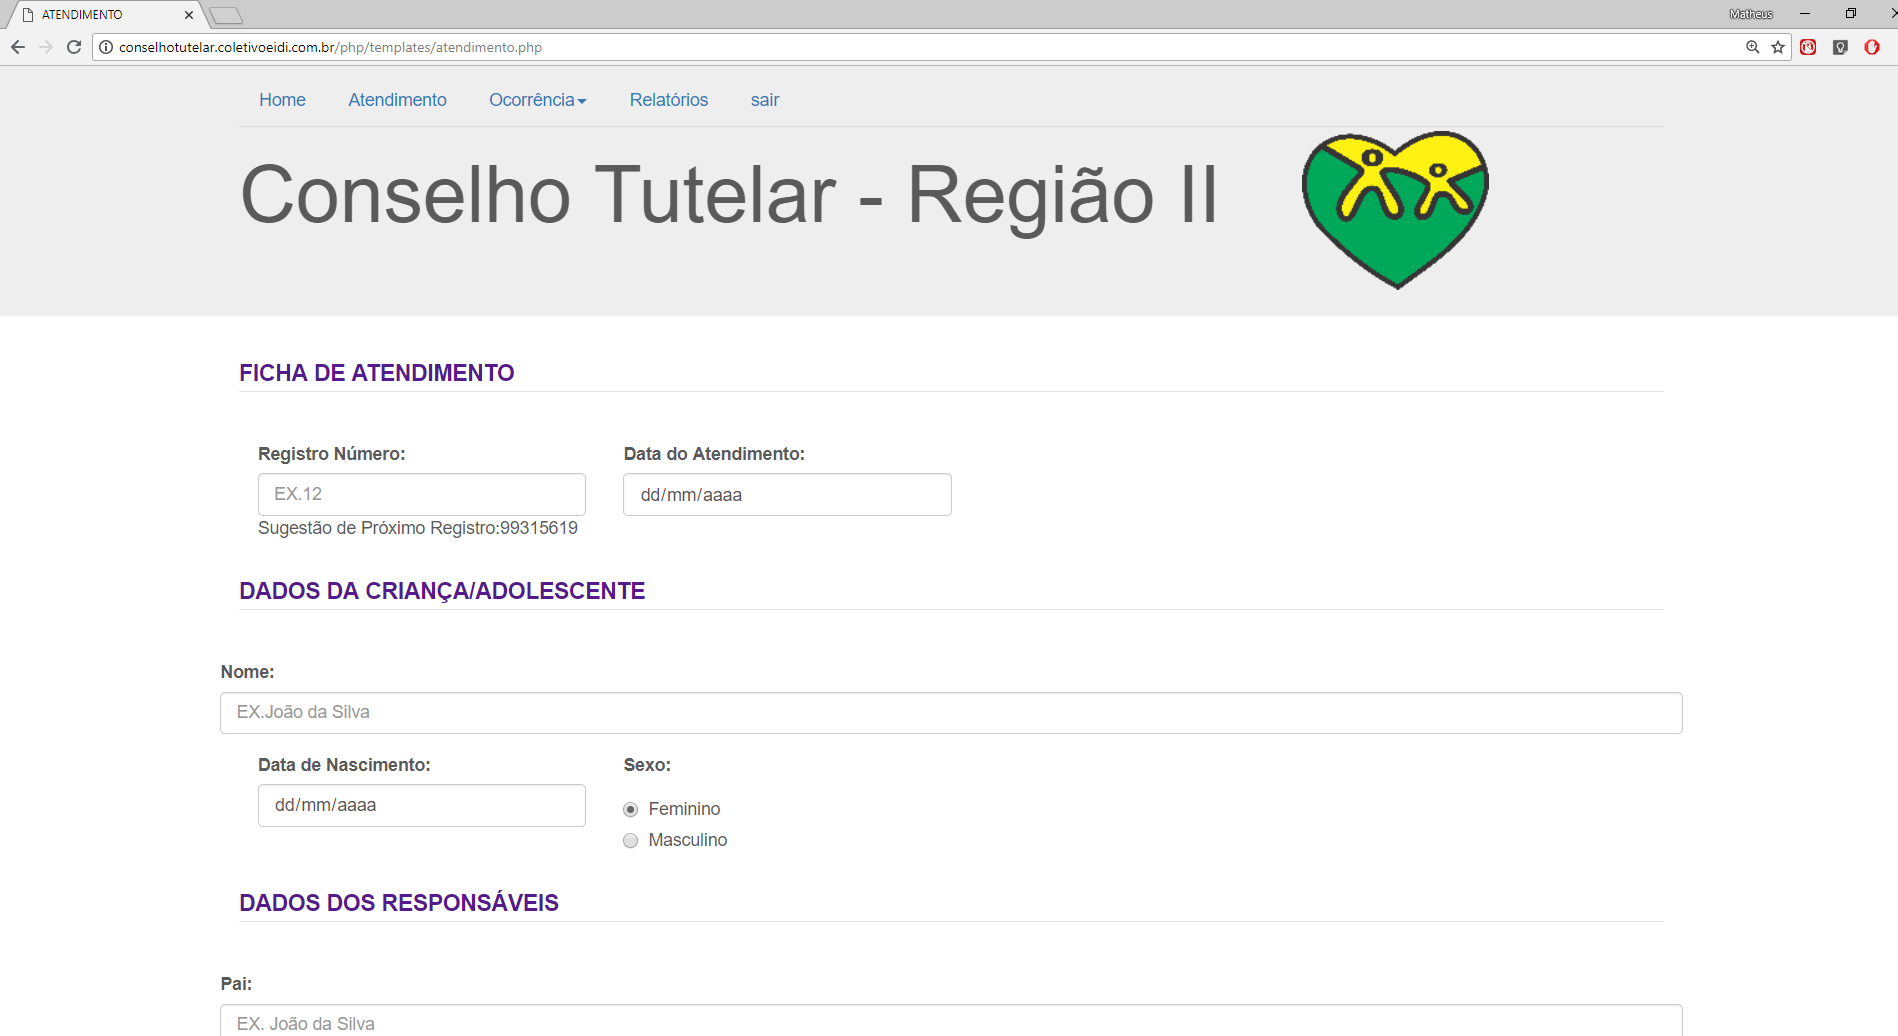
\includegraphics[width=.6\textwidth]{fig/4.png}
\caption{Tela de Atendimento.}
\label{fig:atendimento}
\end{figure}

As telas de ``Concluídas'' e ``Pendentes'', ilustradas na Figura~\ref{fig:pendente}, têm por função listar todas as ocorrências concluídas e pendentes, respectivamente. Em ambas também é possível abrir e/ou editar alguma ficha de atendimento, assim como a geração de PDF das mesmas. Na tela de ``Consulta'', apresentada na Figura~\ref{fig:consulta}, o conselheiro poderá buscar por ocorrências já cadastradas. Caso haja ao menos uma ocorrência, o sistema retornará de acordo com os dados fornecidos. Caso contrário, uma mensagem alertando que nenhuma ocorrência existe para os parâmetros fornecidos.

\begin{figure}[tb]
\begin{center}
	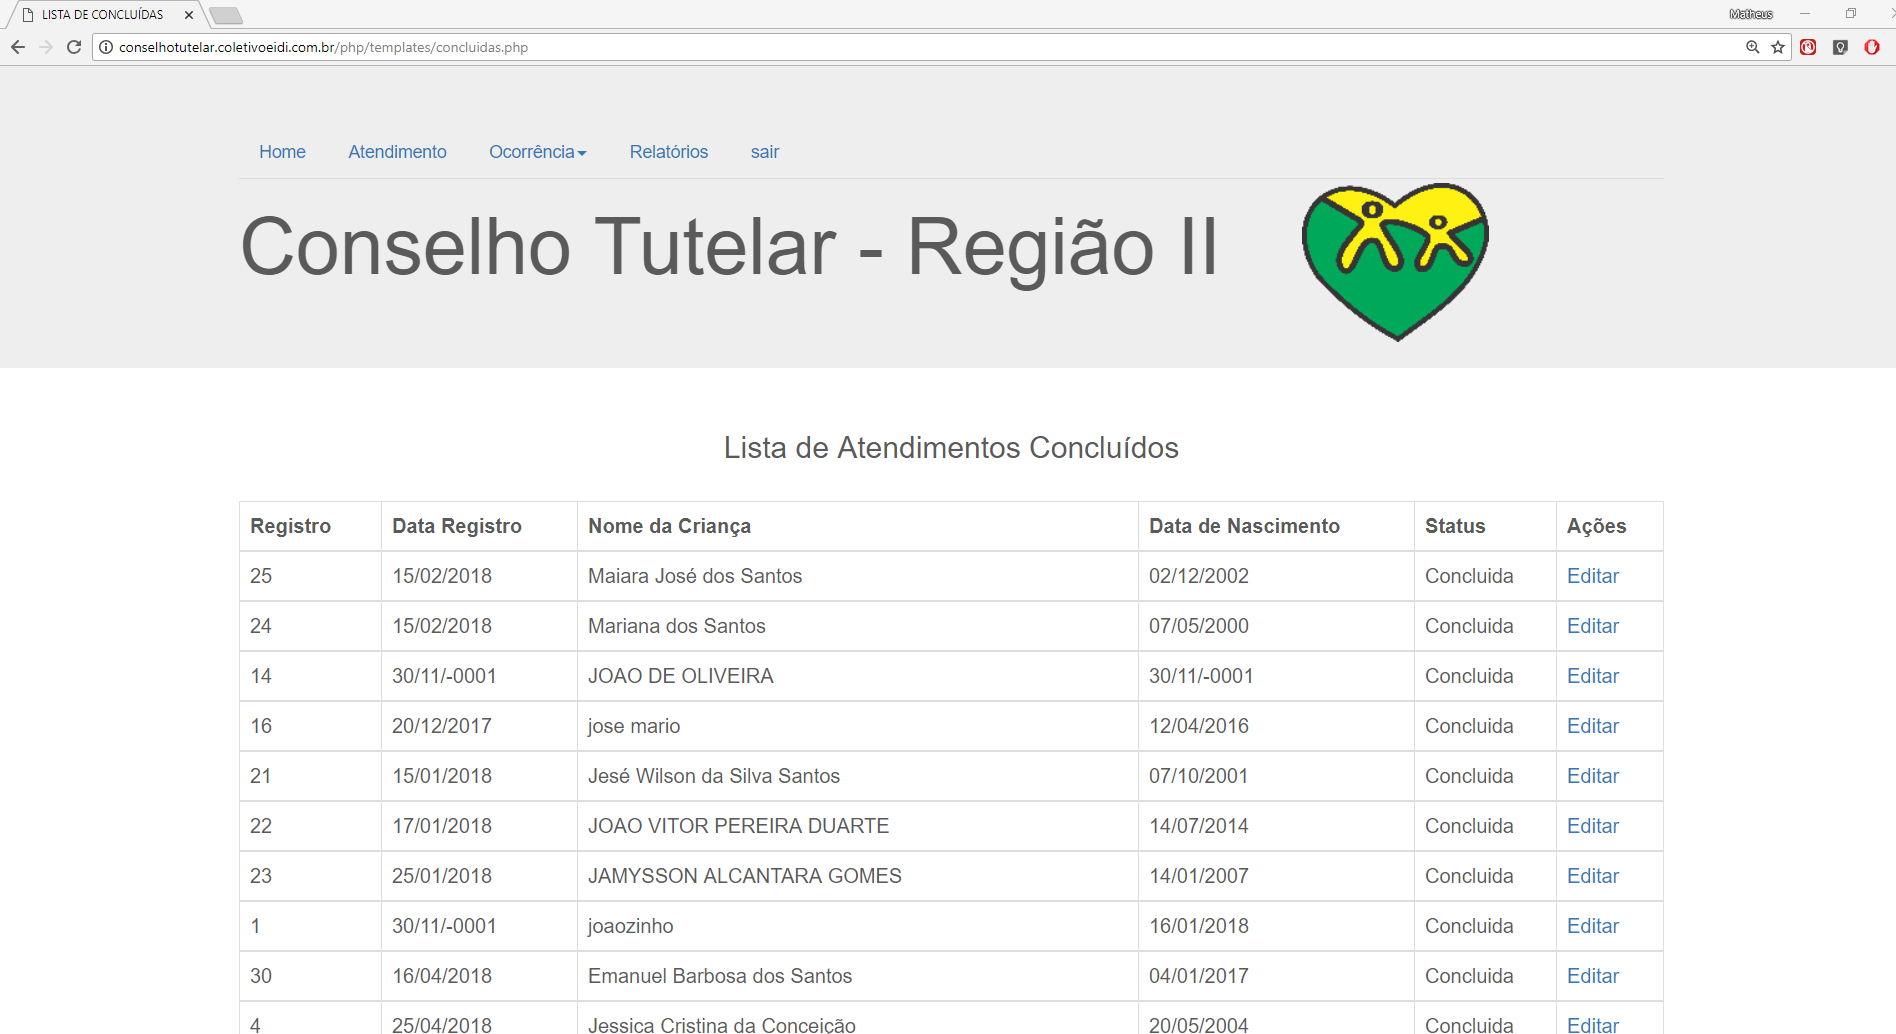
\includegraphics[height=3.5 cm]{fig/6.png} \quad
	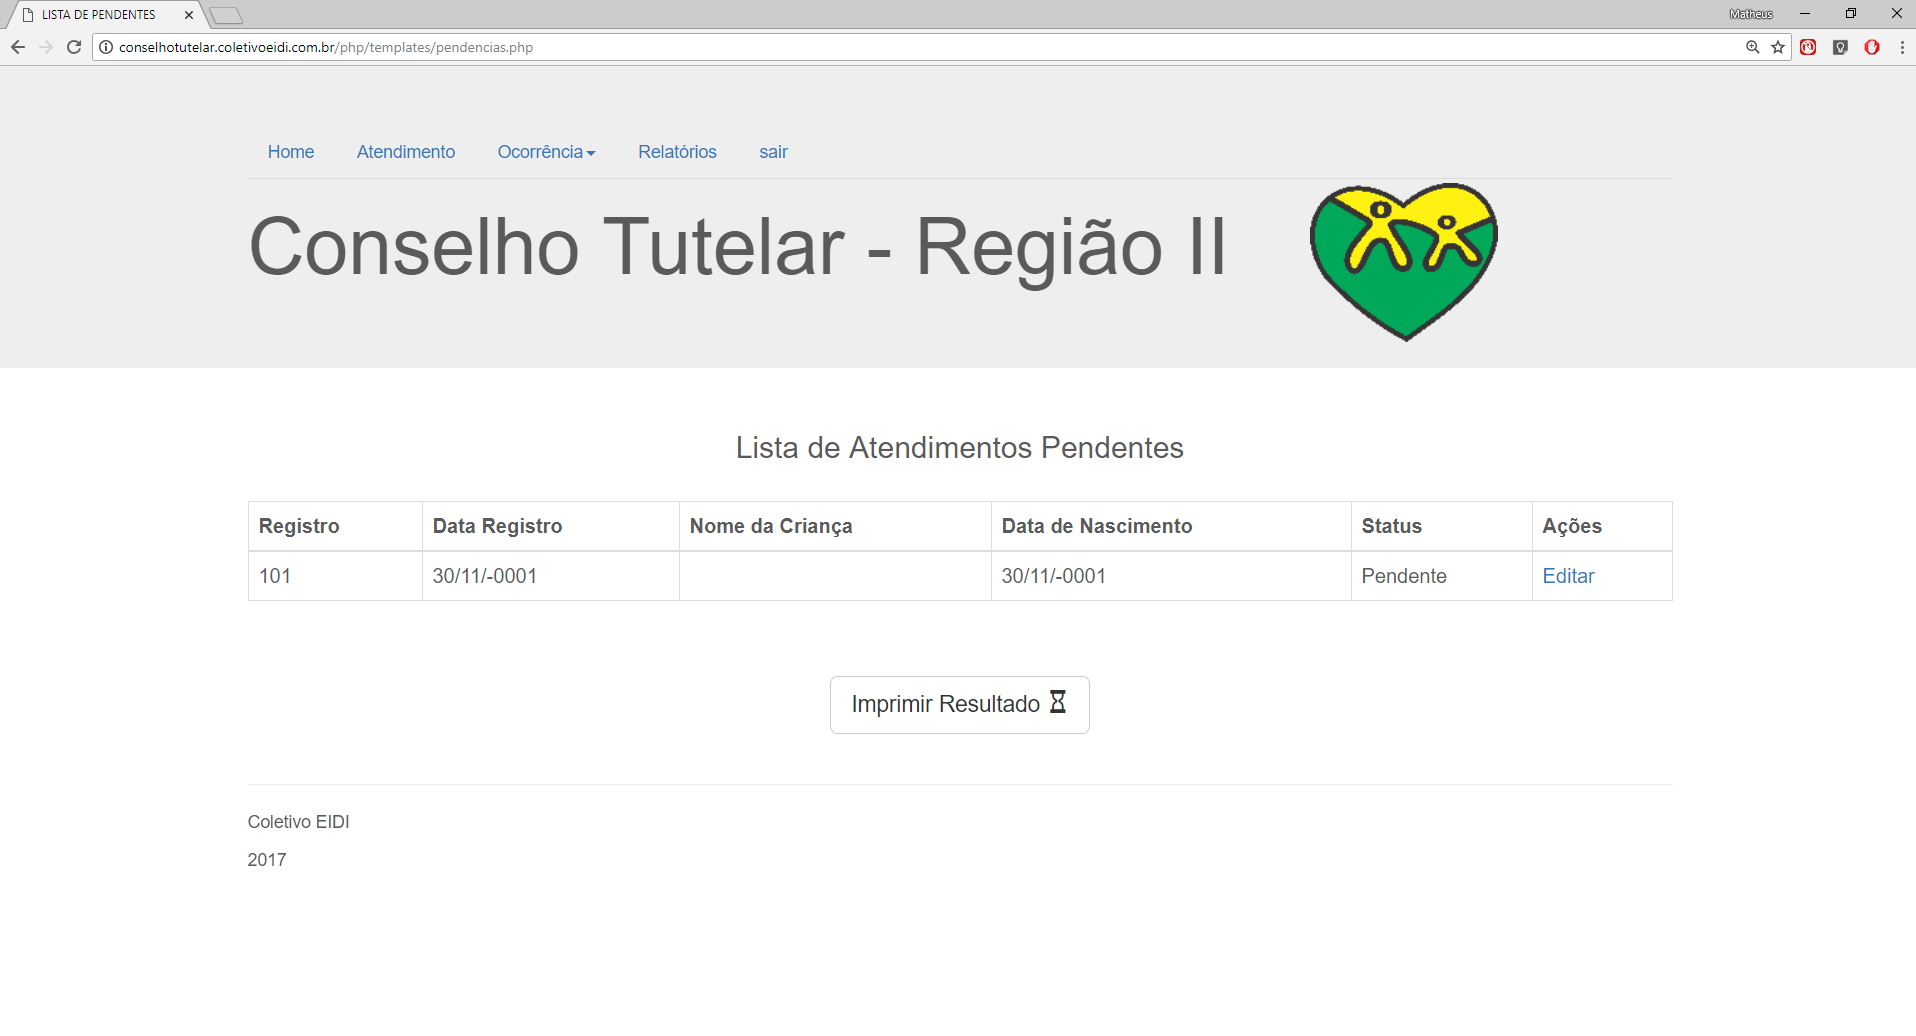
\includegraphics[height=3.5 cm]{fig/7.png}
\caption{Telas de Concluídas e Pendentes, respectivamente. } \label{fig:pendente}
\end{center}
\end{figure}

\begin{figure}[ht]
\centering
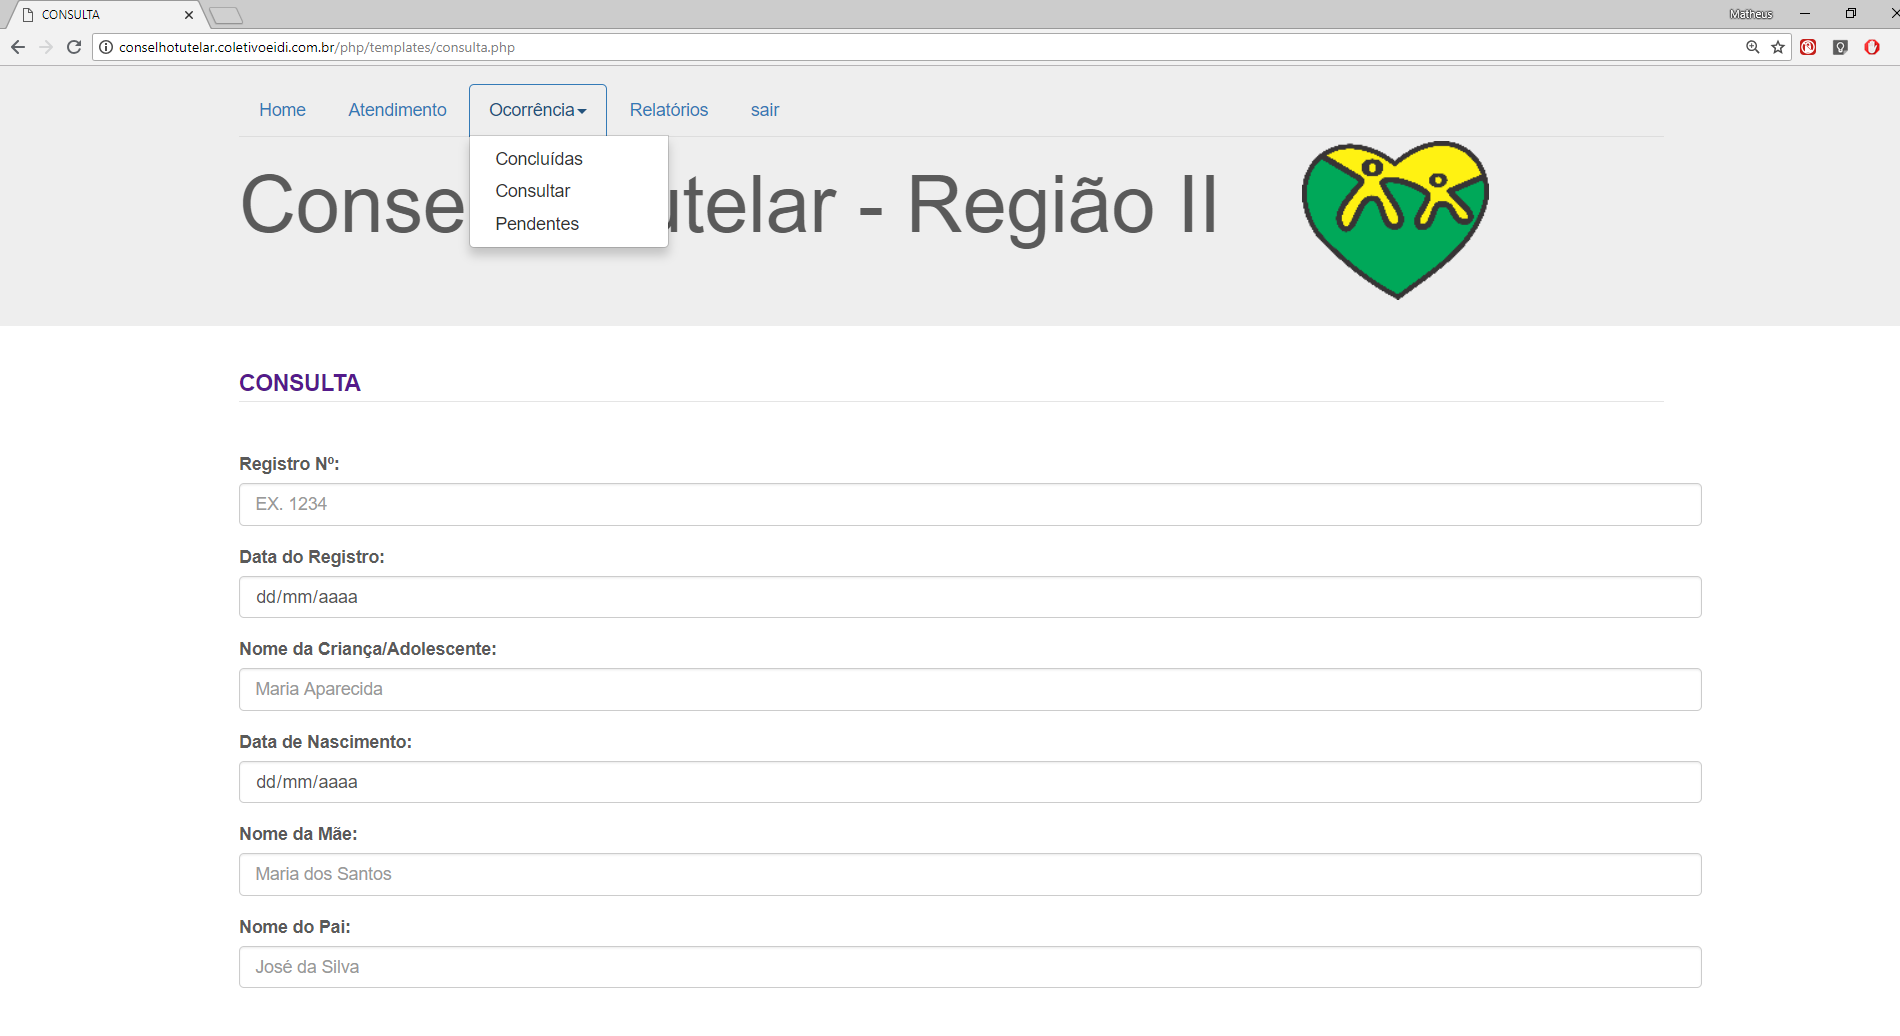
\includegraphics[width=.55\textwidth]{fig/5.png}
\caption{Tela de Consulta.}
\label{fig:consulta}
\end{figure}

Por fim, na tela de ``Relatórios'' (Figura~\ref{fig:relatorio}) o conselheiro irá escolher sobre qual ano ele deseja que seja gerado o relatório. A partir disso, um PDF será gerado com todos os dados referentes aquele ano. Vale ressaltar que os desenhos das fichas de atendimento e do relatório foram feitos de acordo com as fichas que eram feitas manualmente todos os dias pelo Conselho Tutelar.

\begin{figure}[ht]
\centering
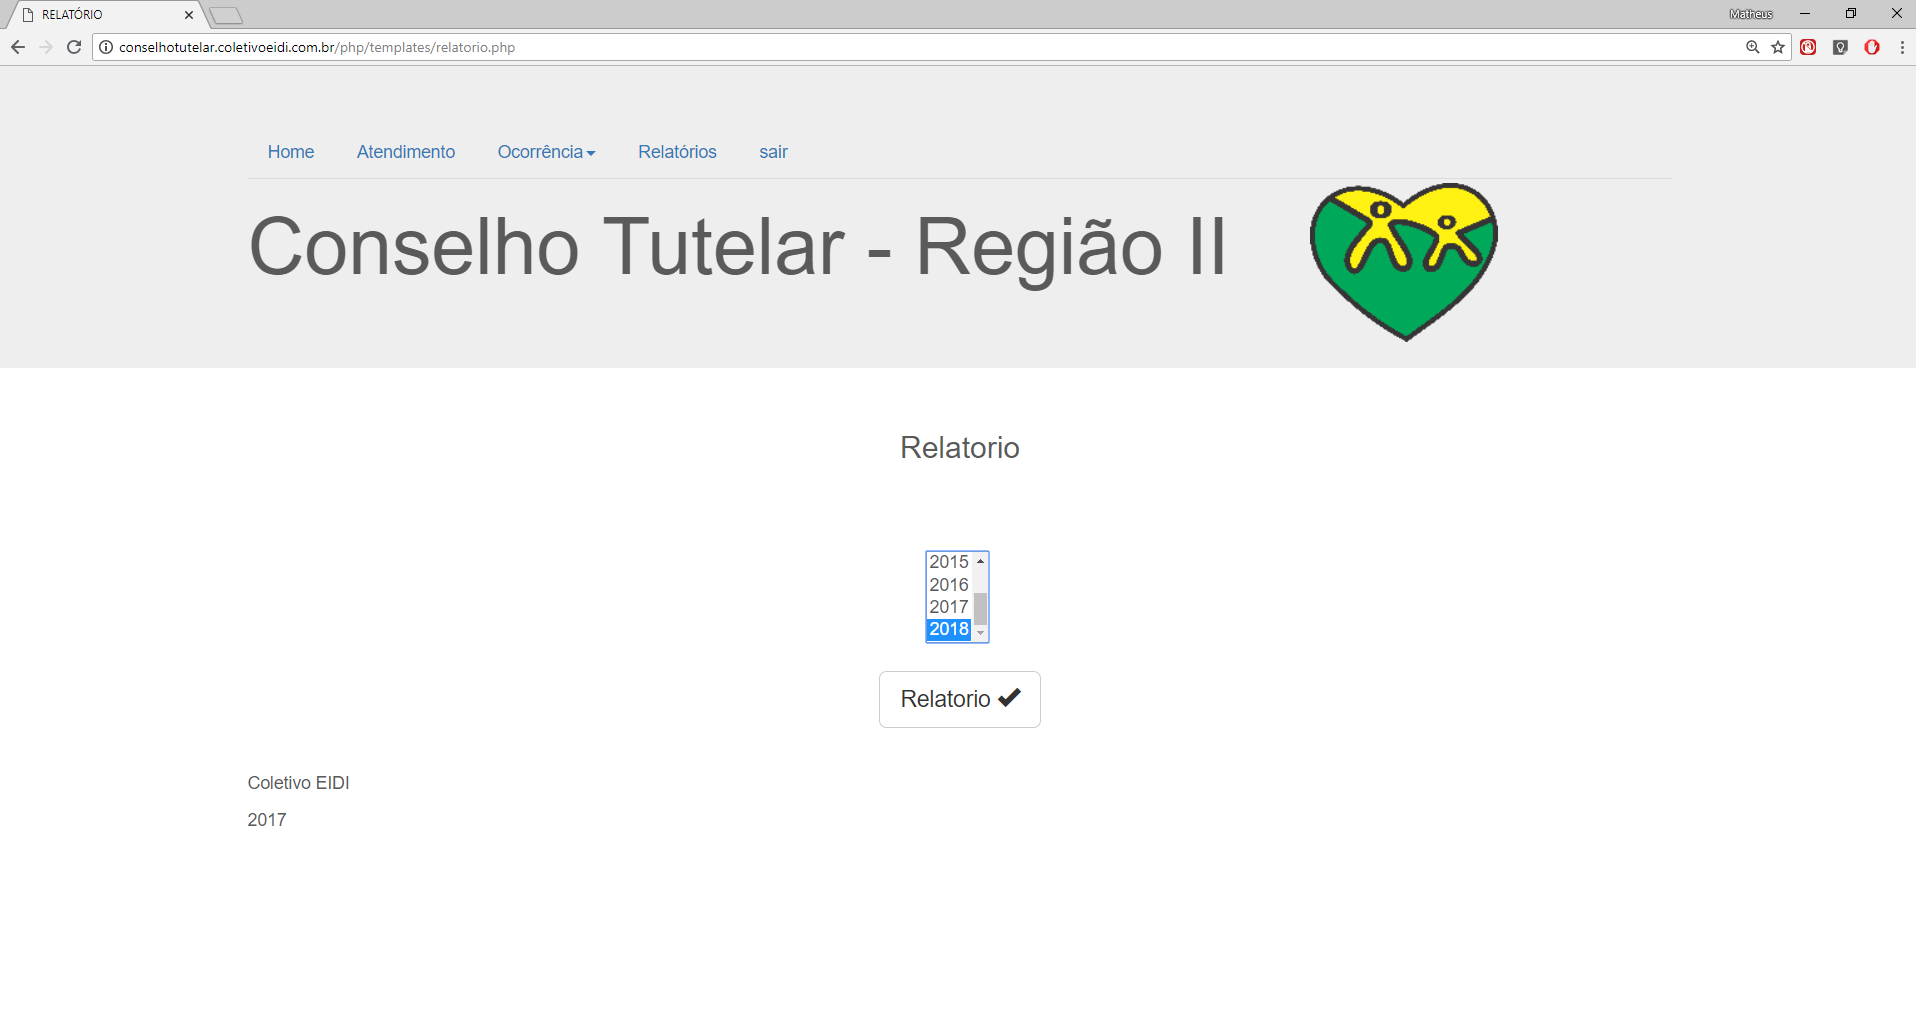
\includegraphics[width=.55\textwidth]{fig/8.png}
\caption{Tela de Relatórios.}
\label{fig:relatorio}
\end{figure}

\section{Conclusão}

Apesar de estar em fase de testes e ainda com alguns recursos a serem implementados, como a mudança da interface e a geração de gráficos a partir dos dados contidos no sistema, o software apresenta resultados iniciais satisfatórios. O sistema está sendo utilizado pelo Conselho Tutelar e, segundo relatos dos próprios conselheiros, muitas atividades estão sendo realizadas mais eficientemente. Contudo, o sistema ainda apresenta alguns problemas, tais como: algumas consultas não retornam ocorrências existentes, e faltam alguns relatórios específicos. 

Considerando que o sistema ainda se encontra em desenvolvimento, os problemas apontados pelos conselheiros são considerados naturais. Tais problemas estão sendo resolvidos. Espera-se que em alguns meses o Conselho Tutelar já esteja usando um sistema estável e livre de \textit{bugs}. Como trabalho futuro, o modelo TAM\footnote{\url{https://is.theorizeit.org/wiki/Technology_acceptance_model}} (\textit{Technology acceptance model}) será implementado, visando avaliar a aceitação do sistema por parte dos conselheiros. 

\bibliographystyle{sbc}
\bibliography{sbc-template}

\end{document}
